\documentclass[a4paper,11pt]{article}

\usepackage[ngerman]{babel}

\usepackage{url}
\usepackage{abstract}
\usepackage{graphicx}
\usepackage{booktabs}
\usepackage{float}
\usepackage{tabularx}
\usepackage{amsmath}
\usepackage{hyperref}
\usepackage{listings}
\usepackage{color}
\usepackage{xcolor}
\usepackage{todonotes}
\usepackage[binary-units]{siunitx}
\usepackage{hyphenat}
\usepackage{fontspec}
%%\usepackage[bottom]{footmisc} breaks referencing of footnotes idk

\usepackage{tgpagella}
\setmainfont{TeX Gyre Pagella}

\usepackage[top=3cm]{geometry}
\usepackage{parskip} %% Absatz anstatt amerikanischer Einrückung

% configure vertical spacing in lists
\usepackage{enumitem}
\setitemize{partopsep=4pt,parsep=2pt}
\setdescription{partopsep=4pt,parsep=6pt}

\makeatletter
\def\namedlabel#1#2{\begingroup
	#2%
	\def\@currentlabel{#2}%
	\phantomsection\label{#1}\endgroup
}
\makeatother

\definecolor{dkgreen}{rgb}{0,0.6,0}
\definecolor{gray}{rgb}{0.5,0.5,0.5}
\definecolor{mauve}{rgb}{0.58,0,0.82}

\lstset{frame=tb,
	language=Java,
	aboveskip=3mm,
	belowskip=3mm,
	showstringspaces=false,
	columns=flexible,
	basicstyle={\small\ttfamily},
	numbers=none,
	numberstyle=\tiny\color{gray},
	keywordstyle=\color{blue},
	commentstyle=\color{dkgreen},
	stringstyle=\color{mauve},
	breaklines=true,
	breakatwhitespace=true,
	tabsize=3
}

\newcommand{\shellcmd}[1]{\texttt{\footnotesize\$ #1}}

\newcommand{\localauthor}[1]{\color{gray} #1 \normalcolor}

\newcommand{\XXitem}[2]{\item[] \textbf{#1} \phantomsection \label{#2}}

\newcommand{\doubletitle}[2]{\title{#1 \\ [1ex] \normalsize #2}}
\newcommand{\extauthor}[2]{\author{#1 \\ \normalsize #2}}

\begin{document}

	\begin{titlepage}
		\centering

		$~$

		\vspace{0.2cm} %% Hack for vspace to work

		\Huge \textbf{Pflichtenheft}\\
		\normalsize Endgültige Abgabe\vspace{0.5cm}

		\Huge Team 2
		\Large

		SEP WS 2021/22

		\vspace{2cm}

		
\includegraphics[width=0.8\linewidth]{graphics/LasEs-logo}

		\vspace{2cm}

		Betreuer:

		\textsc{Prof. Dr. Christian Bachmaier}

		\vspace{1cm}

		\begin{table}[H]
			\centering
			\Large
			\begin{tabular}{ll}
				\toprule
				\textbf{Projektphase} & \textbf{Leiter} \\
				\midrule
				Pflichtenheft & Johann Schicho \\
				Entwurf & Stefanie Gürster \\
				Feinspezifikation & Johannes Garstenauer \\
				Implementierung & Thomas Kirz \\
				Validierung & Sebastian Vogt \\
				\bottomrule
			\end{tabular}
		\end{table}

	\vspace{1cm}

	29. Oktober 2021

	\end{titlepage}

	%%\doubletitle{Pflichtenheft}{SEP WS 2021/22}

	%%\extauthor{Gruppe 2}{Johannes Garstenauer, Stefanie Gürster, Thomas Kirz, Johann Schicho, Sebastian Vogt}

	%%\date{Datum}
	\pagenumbering{gobble}

	%%\maketitle
	\tableofcontents
	%%\listoftodos

	%% ENDE Titelblatt

	\newpage
	\pagenumbering{arabic}

	\section{Einleitung}
	\localauthor{Thomas Kirz}

LasEs ist ein \emph{Submission und Review Management System}, also eine Webseite bei der Wissenschaftler:innen Artikel hochladen können, um von Gutachtern \emph{peer reviewed} zu werden.\\
Auf Basis der Gutachten kann ein \emph{Editor} eines Journals oder einer Konferenz den Artikel für die Veröffentlichung akzeptieren.


	\section{Zielbestimmungen}
	\localauthor{Thomas Kirz}

\subsection{Musskriterien}
Ziel des Projekts ist eine Webapplikation mit Benutzeroberfläche in englischer Sprache, die von mehreren Nutzenden mit verschiedenen Rollen und Rechten benutzt werden kann.
Alle Rollen, außer die anonymen Nutzenden, werden als authentifizierte Nutzende bezeichnet und können Papers einreichen.
Falls sie die Rolle eines Administrators, eines Gutachters oder eines Editors bekleiden, stehen ihnen weitere Funktionen zur Verfügung..

Eine Erweiterung des Systems um Funktionen, die über die folgenden Kriterien hinausgehen, wie z.B.\ das Publizieren von Artikeln, soll einfach möglich sein.

\subsubsection{Administratoren}\label{mkrit:admin}
An oberster Stelle in der Hierarchie stehen die Administratoren mit allumfassenden Rechten, welche als Betreiber der Anwendung fungieren.
Sie konfigurieren das System gemäß den Anforderungen und Wünschen des Betreibers und verwalten Benutzende.
Außerdem richten sie Konferenzen und Journale ein, also Veranstaltungen bzw.\ Zeitschriften, bei denen wissenschaftliche Artikel veröffentlicht werden.
Dafür ernennen sie jeweils Editoren, die die Einreichungen für ihre Konferenzen und Journale verwalten.

\subsubsection{Editoren}\label{mkrit:editor}
Editoren haben die Möglichkeit, weitere Editoren für ein \hyperref[glo:wissForum]{wissenschaftliches Forum} ernennen.
Sie laden Gutachter für das Review von Artikeleinreichungen ein und entscheiden nach Fertigstellung der Gutachten auf dessen Basis, ob sie angenommen oder (mit Begründung) abgelehnt werden sollen.

\subsubsection{Gutachter}\label{mkrit:gutachter}
Gutachter können Einladungen zur Begutachtung einer wissenschaftlichen Arbeit annehmen oder ablehnen.
Nehmen sie diese an, so müssen sie sich spätestens zu diesem Zeitpunkt registrieren.
Danach laden sie das Dokument herunter und erstellen ihren Bericht in einem eigenen PDF-Dokument.
Unter Einhaltung einer vom Editor festgelegten Deadline laden sie dieses hoch.
Außerdem stehen ihnen Tools wie ein Kommentarfeld oder die Möglichkeit, eine Empfehlung abzugeben, zur Verfügung.

\subsubsection{Angemeldete Nutzer}\label{mkrit:angemeldet}
Einreichen kann jeder Wissenschaftler nach Registrierung und Anmeldung am System.
Sie finden mithilfe einer Liste oder Suche eine geeignete Konferenz oder ein Journal.
Dort laden sie ihre Artikel als PDF-Datei hoch versehen sie mit Metainformationen wie Daten der Koautoren.
Dabei haben sie die Möglichkeit, auszusuchen, welcher Editor für die Einreichung verantwortlich sein soll.
Über eine Entscheidung des Editors werden sie per E-Mail benachrichtigt.

\subsubsection{Anonyme Nutzer}\label{mkrit:anon}
Anonyme Nutzer können sich initial nur registrieren und dann erst weitere Funktionen benutzen.


\subsection{Wunschkriterien}

Über die nötigen Funktionen hinaus gibt es noch folgende wünschenswerte Kriterien.

Eine Möglichkeit ist, Gutachter bei der Einreichung unverbindlich vorschlagen zu können.

Weitere Einstellungen zur Personalisierung sind möglich,
zum einen die Anzeige eigener Logos und Farbschemata für Konferenzen und Journale oder auch Avatarbilder für die Nutzerprofile.

Neben direkter Annahme oder Ablehnung einer Einreichung ist das Anfordern einer Revision optional.
Die Einreichung müsste also mit gewünschten Änderungen erneut eingesendet werden, erneut begutachtet und evtl.\ akzeptiert werden.

Für Gutachter kann es die Möglichkeit geben, eigene Gutachten zurückzuziehen und löschen zu lassen.

Schließlich gibt es noch die Möglichkeit, die Webseite zweisprachig auf Englisch und Deutsch anzubieten.

\subsection{Abgrenzungskriterien}

Artikel müssen als PDF-Datei eingereicht werden. Das Hochladen von bspw.\ Word- \hyperref[glo:latex]{\LaTeX}-Dateien ist nicht möglich.
Außerdem können diese Dokumente nicht direkt auf der Webseite angezeigt oder bearbeitet werden;
die Nutzer müssen die Dateien herunterladen und dafür eigene Tools benutzen.

Die Veröffentlichung und Lizenzierung von Artikeln ist keine Funktion der Software,
die Annahme oder Ablehnung ist der letzte Schritt einer Einreichung für LasEs.
Auch Zahlungsabwicklungen werden nicht unterstützt.

Die Webseite ist für Laptops und Desktopgeräte optimiert, es wird keine für mobile Endgeräte nutzerfreundliche Oberfläche gewährleistet.


	\section{Produkteinsatz}
	\localauthor{Thomas Kirz}

\subsection{Anwendungsbereiche \& Zielgruppen}

Die Applikation ermöglicht das Einreichen von Artikeln für Konferenzen und Journale.

Damit richtet sie sich an die einreichenden Wissenschaftler:innen, gutachtende \emph{peers} und Editor:innen, die zu den jeweiligen Konferenzen und Journalen gehören.
Die Wissenschaftler:innen und Gutachter:innen sollten dazu qualifiziert sein, in dem Bereich des Artikels wissenschaftliche Arbeiten schreiben zu können.
Die Editor:innen werden von den Konferenzen und Journalen gestellt und sind in der Lage, über die Annahme einer Einreichung zu entscheiden.

Die Anwendung wird auch von Administrator:innen genutzt, um die Software zu betreiben und zu konfigurieren.
Diese sollten daher Erfahrung mit der Installation, Verwaltung und Wartung von Web- und Datenbankapplikationen haben.
Sie haben auch die Aufgabe, Konferenzen und Journale einzurichten und müssen daher mit deren Repräsentanten in Kontakt stehen.

\subsection{Betriebsbedingungen}

LasEs ist als Webanwendung frei im World Wide Web verfügbar und kann daher von allen Nutzer:innen mit ihren eigenen Endgeräten mit gängigen Browsern weltweit bedient werden.

Die Software ist jederzeit zugänglich bis auf eine von dem/der Administrator:in festgelegte wöchentliche Stunde für Wartungsarbeiten.

Für den Betrieb des Systems sind ein Web- und ein Datenbankserver nötig.
Diese können getrennt sein oder zwei Dienste auf dem gleichen Server.
Dafür kann ein externes Rechenzentrum benutzt werden oder man betreibt einen eigenen Server in einer Umgebung mit adäquater Kühlungs- und Sicherheitsinfrastruktur.

	\section{Produktumgebung}
	\localauthor{Johann Schicho}

Durch die Verwendung von Java ist die serverseitige Ausführung von LasEs
grundsätzlich plattformunabhängig.
Die Verwendung von Anwenderseite setzt nur einen modernen Webbrowser voraus.

\subsection{Hardware}

\begin{itemize}
	\item \textbf{Client:} Computer (PC oder Laptop) mit Internetanschluss, um darauf einen Webbrowser zu verwenden.

	\item \textbf{Server:} Rechner mit Internetanschluss, um darauf Webserver und Datenbankserver laufen zu lassen. Datenbankserver und Webserver können auch auf zwei unterschiedlichen Rechnern ausgeführt werden.

	\phantomsection
	\label{dbspezi}
	Referenzsystem für den Datenbankserver ist der FIM Rechner \texttt{bueno}.\\
	\texttt{\textbf{bueno}} führt PostgreSQL 12.x aus.

	\phantomsection
	\label{spezi}

	Referenzsystem für den Webserver ist der FIM CIP Pool Rechner \texttt{ds9}.\\
	\texttt{\textbf{ds9}} hat folgende Systemspezifikationen:

	\begin{itemize}
		\XXitem{CPU:}{spez:cpu} Intel Core i7-4790 @ 3.60GHz x 8

		\XXitem{RAM:}{spez:ram} 16 GiB

		\XXitem{Festplattenkapazität:}{spez:rom} 256 GiB

		\XXitem{Systemarchitektur:}{spez:arch} 64-bit

		\XXitem{Betriebssystem}{spez:os} Debian GNU/Linux 11 (bullseye)
	\end{itemize}


\end{itemize}

\subsection{Software}

\begin{itemize}

	\item \textbf{Client:} Betriebssystem (Windows, MacOS, Linux, etc.) und ein installierter Webbrowser.

	\begin{itemize}
		\item Google Chrome
		\item Mozilla Firefox
		\item Microsoft Edge
	\end{itemize}

	\item \textbf{Datenbankserver:} Betriebssystem (Windows, Linux, etc.) mit folgenden weiteren Voraussetzungen:

	\begin{itemize}
		\item PostgreSQL 12.x SQL Datenbank Server
	\end{itemize}

	\item \textbf{Anwendungsserver:} Betriebssystem (Windows, Linux, etc.) mit folgenden weiteren Voraussetzungen:

	\begin{itemize}
		\item JDK 16 Installation
		\item JSF Referenzimplementation Mojarra $3.0.1$ (mitgeliefert in der Anwendung)
		\item CDI Framework Weld $4.0.2$ (mitgeliefert in der Anwendung)
		\item JDBC (mitgeliefert in der Anwendung)
		\item Apache Tomcat $10.0.x$ HTTP Webserver
	\end{itemize}

\end{itemize}

	Datenbankserver und Anwendungsserver können auf dem selben Rechner ausgeführt werden. Dazu sind dann beide Server-Softwarevoraussetzungen auf einem System zu installieren.

\subsection{Orgware}

\begin{itemize}
	\item Installation der Softwarevoraussetzungen

	\item Konfiguration der Anwendung (Erstmaliges Starten der Anwendung, Verbindung mit PostgreSQL, Erstellung des Datenbank Schemata)

	\item Internetanschluss für den Webserver, der über das öffentliche \textit{freie} Internet zugänglich ist und Internetanschluss oder lokale Netzwerkverbindung zu dem Datenbankserver.

	\item Verschlüsselte Kommunikation über HTTPS. Verwendung einer statischen IP-Adresse und eines vertrauenswürdigem TLS Zertifikats.

	\item E-Mail-Server mit E-Mail-Konto zur Versendung automatisierter Benachrichtigung.

	\item E-Mail-Client auf Rechner des Benutzers um E-Mails zu anderen Benutzern versenden zu können.
\end{itemize}



	\section{Produktfunktionen}\label{produktfunktionen}
	%todo Erstellen eines Nutzerprofils als admin? -> FW
%todo längere einträge in listen aufsplitten
%todo suchen jeweils mit dropdown
%todo ablehnung -> aus Forum entfernt -> auf startseite des nutzers zu sehen
%todo nutzer einreichung zurücknehmen
\localauthor{Johannes Garstenauer}

Die Funktionalität vom LasEs-System soll nach den Benutzerrollen
%link
\textit{anonymer Nutzer}, \textit{angemeldeter Nutzer}, \textit{Editor}, und
\textit{Administrator} untergliedert werden.

Es gilt darüber hinaus, dass alle Funktionen eines einfachen angemeldeten Nutzers auch den höherrangigen Benutzern, wie Editoren und Administratoren, zur Verfügung stehen. Diese hierarchische Ordnung wird im Folgenden genauer spezifiziert.

\subsection{Anonymer Nutzer}\label{funkt:nutzer}
Anonyme Nutzer sind unauthentifizierte Nutzer, deren Zugriffsrechte sich
auf die Registrierung und Anmeldung im System beschränken.

\subsubsection{Allgemein}
\begin{description}
    \XXitem{/F010/}{funkt:010} Beim Aufruf einer Seite durch einen nicht-angemeldeten Benutzer
    wird dieser auf die Anmeldeseite weitergeleitet und zur
    Anmeldung aufgefordert. Ausgenommen davon ist die Hilfeseite zur Anmeldung und die
    Registrierungsseite.
    \XXitem{/FW020/}{funkt:020} Die Standardsprache des Systems ist abhängig von der im Browser
    eingestellten Sprache. Es werden Deutsch und Englisch angeboten.
    Sonst ist die Standardsprache Englisch. Die Sprache der Anwendung kann über die
    Fußzeile geändert werden.
    \XXitem{/F030/}{funkt:030} Auf den wichtigsten Seiten lassen sich von der Fußzeile aus
    Hilfetexte zu den angebotenen Funktionalitäten und der jeweiligen Rolle
    des Nutzers anzeigen. Hierzu öffnet sich ein neuer Tab.
    \XXitem{/F040/}{funkt:040} Ist eine Ressource über eine URL nicht erreichbar (z.B. weil sie nicht existiert/
     die URL fehlerhaft ist) wird eine Fehlerseite angezeigt.%in ang. nutzer darauf verweisen
\end{description}

\subsubsection{Registration}
\begin{description}
    \XXitem{/F050/}{funkt:050} Ein anonymer Nutzer kann von der Anmeldeseite aus mittels eines
    Buttons auf die Registrierungsseite navigieren.
    \XXitem{/F060/}{funkt:060} Über ein Registrierungsformular wird der Nutzer zur Eingabe seiner
    Daten aufgefordert. Verlangt wird die Eingabe eines Passworts,
    sowie von Vor- und Nachname. Optional ist das Einfügen eines Avatarbildes. Letztlich muss die Emailadresse
    angegeben werden, welche einzigartig im System sein muss. Durch das Absenden des Formulars wird der E-Mail Verifizierungsprozess
    gestartet.
    %link email-ver
    \XXitem{/F070/}{funkt:070} Nach der Registrierung wird eine automatisierte E-Mail
    an die angegebene Mailadresse gesendet. Die Nachricht beinhaltet einen Hinweis auf
    die versuchte Registrierung sowie einen Verifizierungslink, welcher auf eine Seite führt, welche
    die erfolgreiche Registrierung bestätigt. Der Account ist nun registriert. Nach einem Augenblick wird der Nutzer
    auf die Startseite weitergeleitet.
\end{description}

\subsubsection{Anmeldung}
\begin{description}
    \XXitem{/F080/}{funkt:080} Mittels eines Anmeldeformulars erfolgt eine Anmeldung durch korrekte Zugangsdaten.
    Diese umfassen die Mailadresse und das Passwort. Ein anonymer Nutzer wird so zum angemeldeten Benutzer.
    Nach erfolgreicher Anmeldung erfolgt eine Weiterleitung auf die Startseite.
    \XXitem{/F090/}{funkt:090} Von der Anmeldeseite ist es möglich zur Registrierungsseite zu gelangen.
    \XXitem{/F100/}{funkt:100} Über einen Klick auf das Logo der Anwendung gelangt der Nutzer jederzeit
    auf die Seite zur Anmeldung.
\end{description}

\subsection{Angemeldeter Nutzer}
Angemeldete Nutzer haben Zugriff auf die Funktionen
\hyperref[funkt:010]{/F110/}, \hyperref[funkt:020]{/F020/}, \hyperref[funkt:030]{/F030/}.
Nach der Anmeldung \hyperref[funkt:080]{/F080/},
stehen außerdem folgende weitere Funktionen zur Verfügung.

\subsubsection{Allgemein}
\begin{description}
    \XXitem{/F120/}{funkt:120} Bei Zugriff auf die Anmelde- oder Registrierungsseite
    wird auf die Startseite weitergeleitet.
    \XXitem{/F130}{funkt:130} Über einen Button in der Kopfzeile kann ein Logout durchgeführt werden.
    Der nun anonyme Nutzer wird auf die Anmeldeseite weitergeleitet.
    \XXitem{/F140/}{funkt:140} Die Fußzeile ermöglicht eine Navigation zum Impressum.
    \XXitem{/F150/}{funkt:150} Über einen Klick auf das Logo der Anmeldung gelangt ein angemeldeter Nutzer auf die
    Startseite.
\end{description}

\subsubsection{Suche}
\begin{description}
    \XXitem{/F160/}{funkt:160} Über die globale Suche kann ein Nutzer jederzeit seine eigenen Papers und nach wissenschaftlichen Foren,
    suchen. Nach Absenden der Suche wird eine Resultatliste angezeigt. Für Papers werden Name, Datum und Status, für
    wissenschaftliche Foren nur der Name abgebildet. %link /D/
    Sie sind nach Namen sortiert.
    \XXitem{/F170/}{funkt:170} Alle Einträge können anhand der angezeigten Informationen sortiert werden.
    Mit einem Klick auf einen Eintrag wird der Nutzer auf die jeweilige Ansichtseite
    der Ressource navigiert.
    \XXitem{/F180/}{funkt:180} Während der Eeingabe in das Suchfeld werden bis zu 10 mögliche Suchergebnisse in
    einem Dropdown Menü angezeigt.
\end{description}

\subsubsection{Profil}
\begin{description}
    \XXitem{/F190/}{funkt:190} Über die Kopfzeile kann sich ein Benutzer zu seinem Profil navigieren.
    \XXitem{/F200/}{funkt:200} Auf der Profilseite kann der Nutzer alle dynamischen Daten über dieses Profil einsehen,
    Eine Ausnahme hiervon ist das gehashte Passwort. %link /D/
    \XXitem{/F205/}{funkt:205} Auf der eigenen Profilseite kann der Nutzer jedes Datum, %link /D/
    welches über ihn gespeichert ist, persistent verändern.
    \XXitem{/F210/} Bei Änderung der Mailadresse wird der E-Mailverifikationsprozess erneut
    begonnen. Die Mailadresse muss im System einzigartig sein. %link
    \XXitem{/F220/}{funkt:220} Der Nutzer kann auf der eigenen Profilseite ein Avatarbild mit einer maximalen
    Größe von 4MB hochladen oder sein altes Avatarbild entfernen oder austauschen. %link /D/
    \XXitem{/F230/}{funkt:230} Auf der eigenen Profilseite kann der Nutzer sein Profil und alle damit verbundenen persistenten
    Daten löschen. Auch seine Einreichungen werden gelöscht und Gutachter, sowie Editoren dieser
    Einreichung per Mail automatisiert informiert. Bevor die Löschung vollzogen wird, wird dem Nutzer
    eine Warnung über diese Konsequenzen angezeigt.
    \XXitem{/FW240/}{funkt:240} Der Nutzer kann außerdem seinen Arbeitgeber, ein oder mehrere Spezialgebiete
    und sein Geburtsdatum angeben.
\end{description}

\subsubsection{Startseite}
\begin{description}
    \XXitem{/F250/}{funkt:250} Die Startseite ist zu jeder Zeit über die Kopfzeile erreichbar.
    \XXitem{/F260/}{funkt:260} Ein Nutzer bekommt auf der Startseite alle Namen von wissenschaftlichen Foren
    in einer Listensicht angezeigt in denen er aktive Einreichungen hat.
    Die Namen, das Datum und der Status dieser aktiven Einreichungen werden unter den Namen der wissenschaftlichen
    Foren angezeigt.
    \XXitem{/F270/}{funkt:270} Die Einreichungen lassen sich nach Namen und Datum und Status
    der Einreichung sortieren. Die wissenschaftlichen Foren lassen sich nach ihrem Namen sortieren.
    \XXitem{/FW280/}{funkt:280} Die Listen lassen sich nach den Namen der Einträge durchsuchen.
    \XXitem{/F290/}{funkt:290} Durch den Klick auf den Namen eines Eintrags der Liste gelangt man auf die jeweilige Übersichtsseite
    der Einreichung oder auf die Seite des jeweiligen wissenschaftlichen Forums.
\end{description}

\subsubsection{Liste der wissenschaftlichen Foren}
\begin{description}
    \XXitem{/F300/}{funkt:300} In einer Liste werden die Namen von wissenschaftlichen Foren angezeigt.
    \XXitem{/F310/}{funkt:310} Über eine Suchleiste kann nach bestimmten wissenschaftlichen Foren mittels
    ihres Namens gesucht werden.
    \XXitem{/F320/}{funkt:320} Die Einträge lassen sich anhand ihres Namens alphabetisch sortieren.
    \XXitem{/FW330/}{funkt:330} Die Einträge lassen sich anhand des Namens durchsuchen.
    \XXitem{/F340/}{funkt:340} Durch einen Klick auf den Namen eines Eintrags wird man auf die Seite des
    jeweiligen wissenschaftlichen Forums navigiert.
\end{description}

\subsubsection{Wissenschaftliches Forum}
\begin{description}
    \XXitem{/F350/}{funkt:350} Auf der Seite eines wissenschaftlichen Forums werden die zugehörigen wesentlichen Daten
    angezeigt. %link /D/
    \XXitem{/F360/}{funkt:360} Dem Nutzer werden seine eigenen Einreichungen in Form einer Liste mit Namen, Datum und Status
    angezeigt.
    \XXitem{/F370/}{funkt:370} Durch einen Klick auf den Namen einer Einreichung gelangt der Nutzer auf die Übersichtsseite
    dieser Einreichung.
    \XXitem{/F380/}{funkt:380} Die Einträge lassen sich nach Namen, Datum und Status
    der Einreichung sortieren.
    \XXitem{/FW390/}{funkt:390} Die Einträge lassen sich anhand ihres Namens alphabetisch sortieren.
    \XXitem{/F400/}{funkt:400} Der Nutzer kann auf die Seite zur Erstellung einer Einreichung navigieren. Hierbei ist
    das Feld, welches die wissenschaftliche Forum bestimmt wird bei dem eingereicht wird, bereits mit
    dem wissenschaftlichen Forum befüllt von dessen Übersichtsseite aus die Navigation auf diese
    Seite ausgeführt wurde.
\end{description}

\subsubsection{Einreichungserstellung}
\begin{description}
    \XXitem{/F410/}{funkt:410} Der Nutzer kann eine Einreichung im System erstellen. Hierzu gibt er in einem
    Formular die nötigen Informationen wie Namen der Einreichung, Namen und E-Mail Adressen der Ko-Autoren,
    sowie den gewünschten Editor angeben. Der Editor wird nach erfolgreicher Erstellung hierüber durch eine
    automatisierte Mail informiert.
    \XXitem{/F420/}{funkt:420} Der Nutzer lädt seine Einreichung in Form einer PDF hoch. Die Abgabe darf eine Dateigröße
    von 20MB nicht überschreiten und muss im PDF-Format erfolgen.
    \XXitem{/FW430/}{funkt:430} Der Nutzer kann bei Einreichung gewünschte Gutachter vorschlagen.
    \XXitem{/F440/}{funkt:440} Durch Absenden des Formulars wird der Editor des Journals bzw. der Konferenz
    informiert. Das Datum der Einreichung wird auf das Datum zum Zeitpunkt der Einreichung fest-
    gelegt.
    \XXitem{/F450/}{funkt:450} Die Einreichung ist erfolgreich, wenn alle Felder ausgefüllt sind und eine PDF
    hochgeladen wurde. Andernfalls wird der Nutzer über das fehlschlagen informiert.
    \XXitem{/F460/}{funkt:460} Nach der erfolgreichen Einreichungen wird der Nutzer auf die Übersichtsseite der
    Einreichung weitergeleitet.
\end{description}

\subsubsection{Einreichung}
\begin{description}
    \XXitem{/F470/}{funkt:470} Dem Nutzer werden Informationen zu seiner Einreichung angezeigt.
    Hierzu gehören der Status der Einreichung, das Datum der Einreichung, das zugehörige
    Journal bzw. Konferenz, Namen und E-Mail Adressen der Ko-Autoren, sowie ein Download zur Einreichung.
    \XXitem{/F480/}{funkt:480} Außerdem werden die Gutachten in einer
    Liste dargestellt zusammen mit ihrem Erstellungsdatum, Gutachterempfehlung und Download. %link /D/
    \XXitem{} Die Gutachten lassen sich nach Namen und Datum
    des Gutachten sortieren
    \XXitem{/FW490/}{funkt:490}... und nach Namen des Gutachten durchsuchen.
%nav
\end{description}

\subsection{Gutachter}\label{funkt:Gutachter}
Gutachter haben die selben Funktion wie gewöhnliche angemeldete Nutzer. Zusätzlich hierzu kommen
die Folgenden:
%ohne /F/ einreichungsseite alle gutachten sehen

\subsubsection{Startseite}
\begin{description}
    \XXitem{/F500/}{funkt:500} Dem Gutachter werden auf seiner personalisierten Startseite zusätzlich zu den eigenen
    Einreichungen und zugehörigen wissenschaftlichen Foren diejenigen angezeigt für die er als Gutachter
    zugeordnet ist. Diese sind als solche gekennzeichnet.
    Für sie gelten dieselben Funktionalitäten wie für eigene Einreichungen. %link
\end{description}

\subsubsection{Suche}
\begin{description}
    \XXitem{/F510/}{funkt:510} Ein Gutachter kann ebenfalls Einreichungen finden, welcher er als Gutachter
    zugeordnet ist. Diese sind als solche gekennzeichnet.
\end{description}

\subsubsection{Wissenschaftliches Forum}
\begin{description}
    \XXitem{/F520/}{funkt:520} Dem Gutachter werden zusätzlich zu den eigenen Einreichungen diejenigen Einreichungen angezeigt,
    welchen er als Gutachter zugeordnet ist. Für diese Einträge gelten dieselben Funktionalitäten wie für die
    eigenen Einreichungen. %link
\end{description}

\subsubsection{Einreichung}
\begin{description}
    \XXitem{/F530/}{funkt:530} Der Gutachter sieht auf der Übersichtseite einer Einreichung welcher als Gutachter
    zugeordnet ist, diejenigen Gutachten welche er selbst erstellt hat in einer
    Liste mit ihrem Erstellungsdatum, Gutachterempfehlung und Download.
    \XXitem{/F540/}{funkt:540} Der Gutachter hat zusätzlich die Möglichkeit zu einer Einreichung der er als Gutachter zugeordnet ist
    ein Gutachten mittels eines Formulars einzureichen. Hierfür ist eine PDF hoc
    \XXitem{/FW550/}{funkt:550} Auf der Einreichungsseite von Einreichungen denen der Gutachter zugeordnet ist,
    kann er in der Liste eigene eingereichte Gutachten zurückziehen. Hieraufhin werden sie aus
    der Datenbank entfernt und nicht mehr angezeigt.
    \XXitem{/F560/}{funkt:560} Der Einreicher und Editor werden über neue oder entfernte Gutachten mit einer automatisierten
    Mail informiert.
    %einreicher & editor über gutachten informieren
\end{description}

\subsection{Editor}\label{funkt:editor}
Editoren haben Zugriff auf alle Funktionen welche angemeldeten Nutzern zur Verfügung stehen.
Außerdem hat ein Editor die Folgenden zusätzlichen Funktionalitäten:
%keine Editierung von eigenen Einreichungen.
%Hat Profilsichtrechte von Nutzer.

\subsubsection{Startseite}
\begin{description}
    \XXitem{/F570/}{funkt:570} Dem Editor werden auf seiner personalisierten Startseite zusätzlich zu den eigenen
    Einreichungen und zugehörigen wissenschaftlichen Foren diejenigen in einer
    Liste angezeigt welchen er als Editor zugeordnet ist. Sie sind als solche gekennzeichnet.
    Für diese Einträge gelten dieselben Funktionalitäten wie  %link
\end{description}

\subsubsection{Suche}
\begin{description}
    \XXitem{/F580/}{funkt:580} Ein Editor kann ebenfalls Einreichungen finden, welchen er als Editor zugeordnet ist
    Diese sind als solche gekennzeichnet.
    \XXitem{/F590/}{funkt:590} Ein Editor kann ebenfalls Einträge zu allen Nutzern finden.
\end{description}

\subsubsection{Benutzer}
\begin{description}
    \XXitem{/F600/}{funkt:600} Ein Editor kann auf die Nutzerliste über die Kopfzeile zugreifen.
    \XXitem{/F610/}{funkt:610} Hier werden ihm alle Nutzer mit Namen und E-Mail übersichtlich in einer Liste angezeigt.
    \XXitem{/F620/}{funkt:620} Diese Liste kann alphabetisch nach Namen und Mailaddresse sortiert werden.
    \XXitem{/FW630/} Die Liste kann anhand von Namen und Mailadresse durchsucht werden.
    \XXitem{/F640/}{funkt:640} Mit einem Klick auf einen Eintrag wird der Editor auf das zugehörige Profil navigiert.
\end{description}

\subsubsection{Wissenschaftliches Forum}
\begin{description}
    \XXitem{/F650/}{funkt:650} Einem Editor werden auf der Publikationsseite einer Konferenz bzw. eines Journals für
    welches er als Editor fungiert alle aktiven Einreichungen in einer Liste dargestellt.
    Solche bei denen er als Editor eingesetzt wird werden als solche gekennzeichnet.
    Für diese Einträge gelten dieselben Funktionalitäten wie für die eigenen Einreichungen. %link
    \XXitem{/F660/}{funkt:660} Ein Editor kann andere Editoren ernennen indem er sie mittels ihrer Mailadresse identifiziert.
    Diese müssen bereits als Nutzer registriert sein.
    \XXitem{/F670/}{funkt:670} Ein Editor kann anderen Editoren den Status als Editor aberkennen.
\end{description}

\subsubsection{Einreichung}
\begin{description}
    \XXitem{/F680/}{funkt:680} Ein Editor kann auf der Seite einer Einreichung, welcher er als Editor zugeordnet ist,
    in einem Formular Gutachter zuweisen. Hierzu gibt er deren E-Mail Adressen an.
    %FW Nutzersuche (registrierte Nutzerliste durchsuchbar)
    \XXitem{/F690/}{funkt:690} Wird eine E-Mail Adresse als Gutachter angegeben, so wird nach Absenden des Formulars
    eine automatisierte Mail an diese Adresse versendet. Sie enthält eine Nachricht mit den relevanten
    Informationen zu Einreichung, wissenschaftlichem Forum, sowie
    \begin{itemize}
        \item ... einen Link zur \textbf{Annahme der Begutachtungsanfrage} welcher, sobald geklickt,
        auf die Loginseite verweist auf der eine Nachricht des Dankes anzeigt und zur Anmeldung bzw.
        Registrierung auffordert.
        \item ... einen Mailto-Link zur \textbf{Ablehnung der Begutachtungsanfrage} welcher, sobald
        geklickt, einen Mailentwurf öffnet mit vorausgefülltem Empfänger (zugehöriger Editor)
        und einem Infotext in welchen ein Ablehnungsgrundes eingefügt werden kann.
        Abgesehen hiervon wird zusätzlich eine automatisierte Mail an den Editor versendet in der er
        kurz über die Ablehnung informiert wird, falls die obige E-Mail nie versendet wird.
    \end{itemize}
    \XXitem{/F700/}{funkt:700} Ein Editor kann über Einreichungen eine Annahmeentscheidung treffen. Über diese werden
    beteiligte Gutachter, der Einreicher und beteiligte Ko-Autoren per automatisierter Mail benachrichtigt.
\end{description}

\subsection{Administrator}
Der Administrator besitzt zu Verwaltungszwecken alle Rechte, welche auch Nutzern, Editoren
und Gutachtern zustehen. %Genau genug definiert?
Einem Administrator werden in Listen grundsätzlich alle aktiven Einträge angezeigt.
%UserList editor linken
%Das ausgliedern in /F/s? oder einfach verlinken der /F/s? -> oder von fall zu fall je nachdem
%/F/ hier aussagekräftig ist.
% Einreichungsseite selbe Recht wie Gutachter oder Editor zu verwaltungsszwecken.
\subsubsection{Suche}
\begin{description}
    \XXitem{/F710/}{funkt:710} Ein Administrator kann in der globalen Suche ebenfalls alle Nutzer finden.
    \XXitem{/F720/}{funkt:720} Ein Administrator kann alle vorhandenen Einreichungen finden.
\end{description}

\subsection{Wissenschaftliches Forum}
\begin{description}
    \XXitem{/F730/}{funkt:730} Einem Administrator werden auf der Publikationsseite einer Konferenz bzw. eines Journals
    alle aktiven Einreichungen in einer Liste dargestellt.
    Für diese Einträge gelten dieselben Funktionalitäten wie für eigene Einreichungen. %link
\end{description}

\subsubsection{Profil}
\begin{description}
    \XXitem{/F740/}{funkt:740} Ein Administrator kann einen anderen Nutzer auf dessen Profilseite zum Administrator ernennen.
    \XXitem{/F750/}{funkt:750} Ein Administrator kann einem anderen Administrator auf dessen Profilseite seine
    Administratorrolle aberkennen.
    \XXitem{/FW760/}{funkt:760} Vor dem An- oder Aberkennen von Administratorrechten ist eine gültige
    Passworteingabe erforderlich.
    \XXitem{/F770/}{funkt:770} Der Administrator besitzt auf allen Profilseiten dieselben Rechte zur Änderung
    der persistierten Daten wie ein Nutzer auf seiner eigenen Profilseite. %link
\end{description}

\subsection{Liste der Wissenschaftlichen Foren}
\begin{description}
    \XXitem{/F780/}{funkt:780} Auf dieser Seite kann der Administrator zur Seite navigieren auf welcher er ein neues
    wissenschaftliches Forum anlegen kann. %link
\end{description}

\subsubsection{Erstellung wissenschaftlicher Foren}
\begin{description}
    \XXitem{/F790/}{funkt:790} Auf der Seite zum Erstellen eines wissenschaftlichen Forums kann der Administrator dessen
    wesentliche Daten nach /D/ %link
    festlegen. Bei der Angabe von Editoren wird überprüft, dass diese bereits als Nutzer im System registriert sind.
    Der Name des Forums muss ebenfalls einzigartig sein.
    Nach erfolgreicher Erstellung wird der Administrator auf die Seite dieses wissenschaftlichen Forums
    navigiert.
\end{description}

\subsection{Wissenschaftliches Forum}
\begin{description}
    \XXitem{/F800/}{funkt:800} Auf der Seite eines wissenschaftlichen Forums kann der Administrator alle wesentlichen Daten
    verändern. Insbesondere erfolgt hierbei die Ernennung von Editoren, welche bereits im System
    registriert sein  müssen. Der Name des wissenschaftlichen Forums muss einzigartig sein.
    \XXitem{/FW810/}{funkt:810} Der Administrator kann den Look des wissenschaftlichen Forums durch die folgenden Daten
    verändern. %link
    \XXitem{/F820/}{funkt:820} Auf der Seite eines wissenschaftlichen Forums kann der Administrator diese aus dem System zu löschen.
    Hierbei wird er dazu aufgefordert seine Entscheidung ein zweites Mal zu bestätigen.
    Daraufhin werden alle zugehörigen Daten /D/ und Einreichungen aus dem System entfernt. %link /D/
    %link
\end{description}

\subsection{Konfiguration}
\begin{description}
    \XXitem{/F830/}{funkt:830} Ein Administrator kann auf der Konfigurationsseite den vom Betreiber gewünschten
    'Look and Feel' des Systems festlegen. Hierzu bestimmt der die Daten wie in /D/ definiert. %link
\end{description}

	\section{Produktdaten}
	\localauthor{Sebastian Vogt}

Die Notation \texttt{/DXXX/} erlaubt eine spätere Referenzierung der einzelnen Produktdaten in diesem und weiteren
Dokumenten. \texttt{/DXXX/} steht dabei für ein Musskriterium, \texttt{/DWXXX/} für ein Wunschkriterium. \texttt{XXX} entspricht dabei immer einer dreistelligen Zahl.

\begin{description}
	\XXitem{/D010/}{d010} Für jeden \emph{Nutzer} sind folgende Informationen gespeichert: \hyperref[funkt:nutzer]{Nutzerrolle}, Titel, Vorname, Nachname, E-Mail Adresse, sowie die Menge aller \hyperref[d025]{Einreichungen}.

	\XXitem{/DW015/}{d015} Für jeden Nutzer wird darüber hinaus Arbeitgeber, Spezialgebiet und Geburtsdatum abgespeichert. Siehe \hyperref[funkt:240]{/FW240/}

	\XXitem{/D020/}{d020} Für jedes \emph{Manuskript} sind folgende Informationen abgespeichert: Der Titel, die Namen und E-Mail Adressen der Co-Autoren und die zugehörige PDF Datei.

	\XXitem{/D025/}{d025} Für jede \emph{Einreichung} wird das zugehörige \hyperref[d020]{Manuskript}, der Zeitpunkt der Einreichung, das zugehörige \hyperref[d030]{wissenschaftliche Forum}, der \hyperref[funkt:editor]{Editor} der Einreichung, der Status der Einreichung (\emph{schwarz}: Eingereicht, \emph{gelb}: Revision verlangt, \emph{rot}: Abgelehnt, \emph{grün}: Angenommen), die Gutachter, die Abgabefrist für \hyperref[d040]{Gutachten} und die abgegebenen \hyperref[d040]{Gutachten} gespeichert.

	\XXitem{/DW021/}{d021} Für jede \emph{Einreichung} sind zusätzlich folgende Informationen abgespeichert: Frist für das Einreichen einer erneuten Revision, alle Revisionen (in Form von \hyperref[d020]{Manuskripten}) und die Information, ob diese Revisionen bereits für die Gutachter freigeschaltet sind.

	\XXitem{/DW022/}{d022} Ein \emph{Einreichung} speichert zusätzlich, welche Nutzer als Gutacher:innen vorgeschlagen sind. Diese Werden mit Vorname, Nachname und E-Mail Adresse gespeichert, da sie nicht als Nutzer in der Datenbank existieren müssen.

	\XXitem{/D030/}{d030} Für jedes \emph{wissenschaftliche Forum} ist der Name, die zugehörigen Editoren (mit deren Emailadressen), die Deadline für \hyperref[d025]{Einreichungen}, eine Kurzbeschreibung, eine URL zur Website des Forums und eine Anleitung zur Begutachtung gespeichert.

	\XXitem{/D040/}{d040} Für jedes \emph{Gutachten} wird der Inhalt des Gutachtens als PDF gespeichert, ein Kommentar als Freitext und zusätzlich noch der zugehörige \hyperref[funkt:Gutachter]{Gutachter} und die zugehörige \hyperref[d025]{Einreichung} und ob das Gutachten zur Ansicht für den Einreicher freigschaltet ist.

	\XXitem{/D050/}{d050} Systemweit ist das Logo und der Name der betreibenden Einrichtung, das Farbschema der Kopf- und Fußzeile und das Impressum gespeichert.

	\XXitem{/DW051/}{d051} Die gespeicherten Informationen aus \hyperref[d050]{/D050/} sind für jedes \hyperref[d030]{wissenschaftliche Forum} separat gespeichert.
\end{description}

	\section{Produktleistungen}
	\localauthor{Johann Schicho}

\subsection{Skalierbarkeit}

\begin{description}

	\XXitem{/L010/}{leist:10} Die Anwendung wird bis zu 100000 verschiedene Nutzer und 2000 verschiedene Konferenzen und Journale verwalten können.

	\XXitem{/L020/}{leist:20} Die Anwendung wird bis zu 50 gleichzeitig angemeldete und auf der Webanwendung agierende Nutzer verarbeiten können. Dabei wird die Reaktionszeit jeglicher Nutzerinteraktion mit der Webanwendung nicht mehr als 3 Sekunden dauern. Ausnahme davon ist die allgemeine Suchfunktion, die nicht mehr als 5 Sekunden dauert, um ein Ergebnis anzuzeigen.

\end{description}

\subsection{Usability}

\begin{description}
	\XXitem{/L030/}{leist:30} Die Benutzeroberfläche ist intuitiv zu bedienen sein und zeigt pro Seite nur gezielt Informationen, die der Nutzer sehen will, und ist nicht überladen.

	\XXitem{/L040/}{leist:40} Lange Listen werden paginiert. Das heißt sie sind über mehrere Seiten aufgeteilt. Ein solcher Umbruch findet nach je 25 Listeneinträgen statt. Durch Anklicken eines Listeneintrags wird dann auf die zugehörige Übersichtsseite weitergeleitet.

	\XXitem{/L042/}{leist:042} Listen werden filterbar sein. Eine Spalte kann also auf einen bestimmten Wert gefiltert werden.

	\XXitem{/L045/}{leist:045} Alle Listen sind nach ihren Spalten auf- oder absteigend sortierbar.

	\XXitem{/L050/}{leist:050} Über die Kopfzeile, die auf jeder nach dem Login vorzufindenden Seite der Webanwendung
	vorhanden ist, steht eine Suchfunktion zur Verfügung.

	\XXitem{/L055/}{leist:055} Über \emph{Tooltips} kann zu wesentlichen Funktionen der Anwendung eine Kurzhilfe eingeblendet werden. Damit können etwaige Fragen der Nutzer geklärt werden.

	\XXitem{/L060/}{leist:60} Bei fehlerhaften Eingaben wird der Nutzer informiert und kann diese ohne erneutes Eingeben korrigieren, da sie stehen bleiben. Eine Ausnahme ist die Eingabe eines neues Passworts.

	\XXitem{/L062/}{leist:062} Nach erfolgreichen Datenänderungen wird der Nutzer darüber in kurzen Hinweistexten informiert.

	\XXitem{/L065/}{leist:65} Die Verwendung von Cookies ist nicht zwingend erforderlich.
\end{description}

\subsection{Datensicherheit}

\begin{description}
	\XXitem{/L070/}{leist:070} Alle in der Anwendung erfassten Daten werden in der PostgreSQL Datenbank persistent abgelegt.

	\XXitem{/L080/}{leist:080} Die Konsistenz der Daten über Änderungen hinweg wird durch Transaktionen sichergestellt.

	\XXitem{/L090/}{leist:090} Sollten durch Löschen bestimmter Datensätze davon abhängige weitere Datensätze gelöscht werden, wird der Nutzer vorher deutlich gewarnt.
\end{description}

\subsection{Datenschutz}

\begin{description}
	\XXitem{/L100/}{leist:100} Es wird sichergestellt, dass keine sensiblen Daten für unberechtigte Dritte zugänglich sind.

	\XXitem{/L110/}{leist:110} Alle personenbezogenen Daten werden, wie Nutzerdaten und Passwörter werden über eine verschlüsselte HTTPS Verbindung übertragen.

	\XXitem{/L120/}{leist:120} Der \hyperref[funkt:080]{Login} in das System ist über die Emailadresse und Passwort möglich.

	\XXitem{/L130/}{leist:130} Das Passwort muss 8-100 Zeichen lang sein und mindestens Groß- und Kleinbuchstaben, Zahlen und Sonderzeichen enthalten.

	\XXitem{/L140/}{leist:140} Die Registrierung muss durch eine \hyperref[funkt:060]{Bestätigungsemail}, die an die vom Nutzer angegebene Email-Adresse gesendet wird, authentifiziert werden.

	\XXitem{/L142/}{leist:142} Bei Änderung der hinterlegten Email-Adresse muss diese ebenfalls bestätigt werden. Dazu wird eine Bestätigungsemail an die neue Email-Adresse gesendet.
\end{description}

\subsection{Logging}

\begin{description}
	\XXitem{/L145/}{leist:145} Das System verfügt über einen detaillierten Logger, der alle Fehler und Events während der Laufzeit des Systems sammelt. Hierbei werden die Fehler in 3 verschiedene Fehlerklassen eingeteilt: \emph{Error}, \emph{Warning} und \emph{Debug}.
\end{description}

\subsection{Internationalisierbarkeit}

\begin{description}
	\XXitem{/L150/}{leist:150} Die Texte auf der Website werden in UTF-8 kodiert
	und ausgeliefert, um \textit{Internationalization (i18n)} in verschiedenen Sprachen zu ermöglichen.

	\XXitem{/L155/}{leist:155} Die Standard Sprache der Webanwendung ist Englisch.

	\XXitem{/WL160/}{leist:160} Die \hyperref[funkt:020]{mehrsprachige Implementierung} umfasst Englisch und Deutsch.
 \end{description}

\subsection{Installation}

\begin{description}
	\XXitem{/L170/}{leist:170} Es gibt eine kurze Installationsanleitung\footnote{Siehe mitgelieferte INSTALL.txt} für den Systemadministrator. Diese leitet weiter auf Installationsbeschreibungen der einzelnen Softwarevoraussetzungen.

	\XXitem{/L180/}{leist:180} Die Erstinbetriebnahme soll die Möglichkeit bieten, die benötigten Datenbankschemata automatisch zu erstellen.
\end{description}


	\section{Benutzeroberfläche}
	\localauthor{Stefanie Gürster}
\subsection{Benutzerfluss}
Im Folgenden werden funktionale Aussagen über die Benutzeroberfläche, mithilfe eines Benutzerflussdiagramms, getroffen.

\begin{figure}[H]
	\centering
	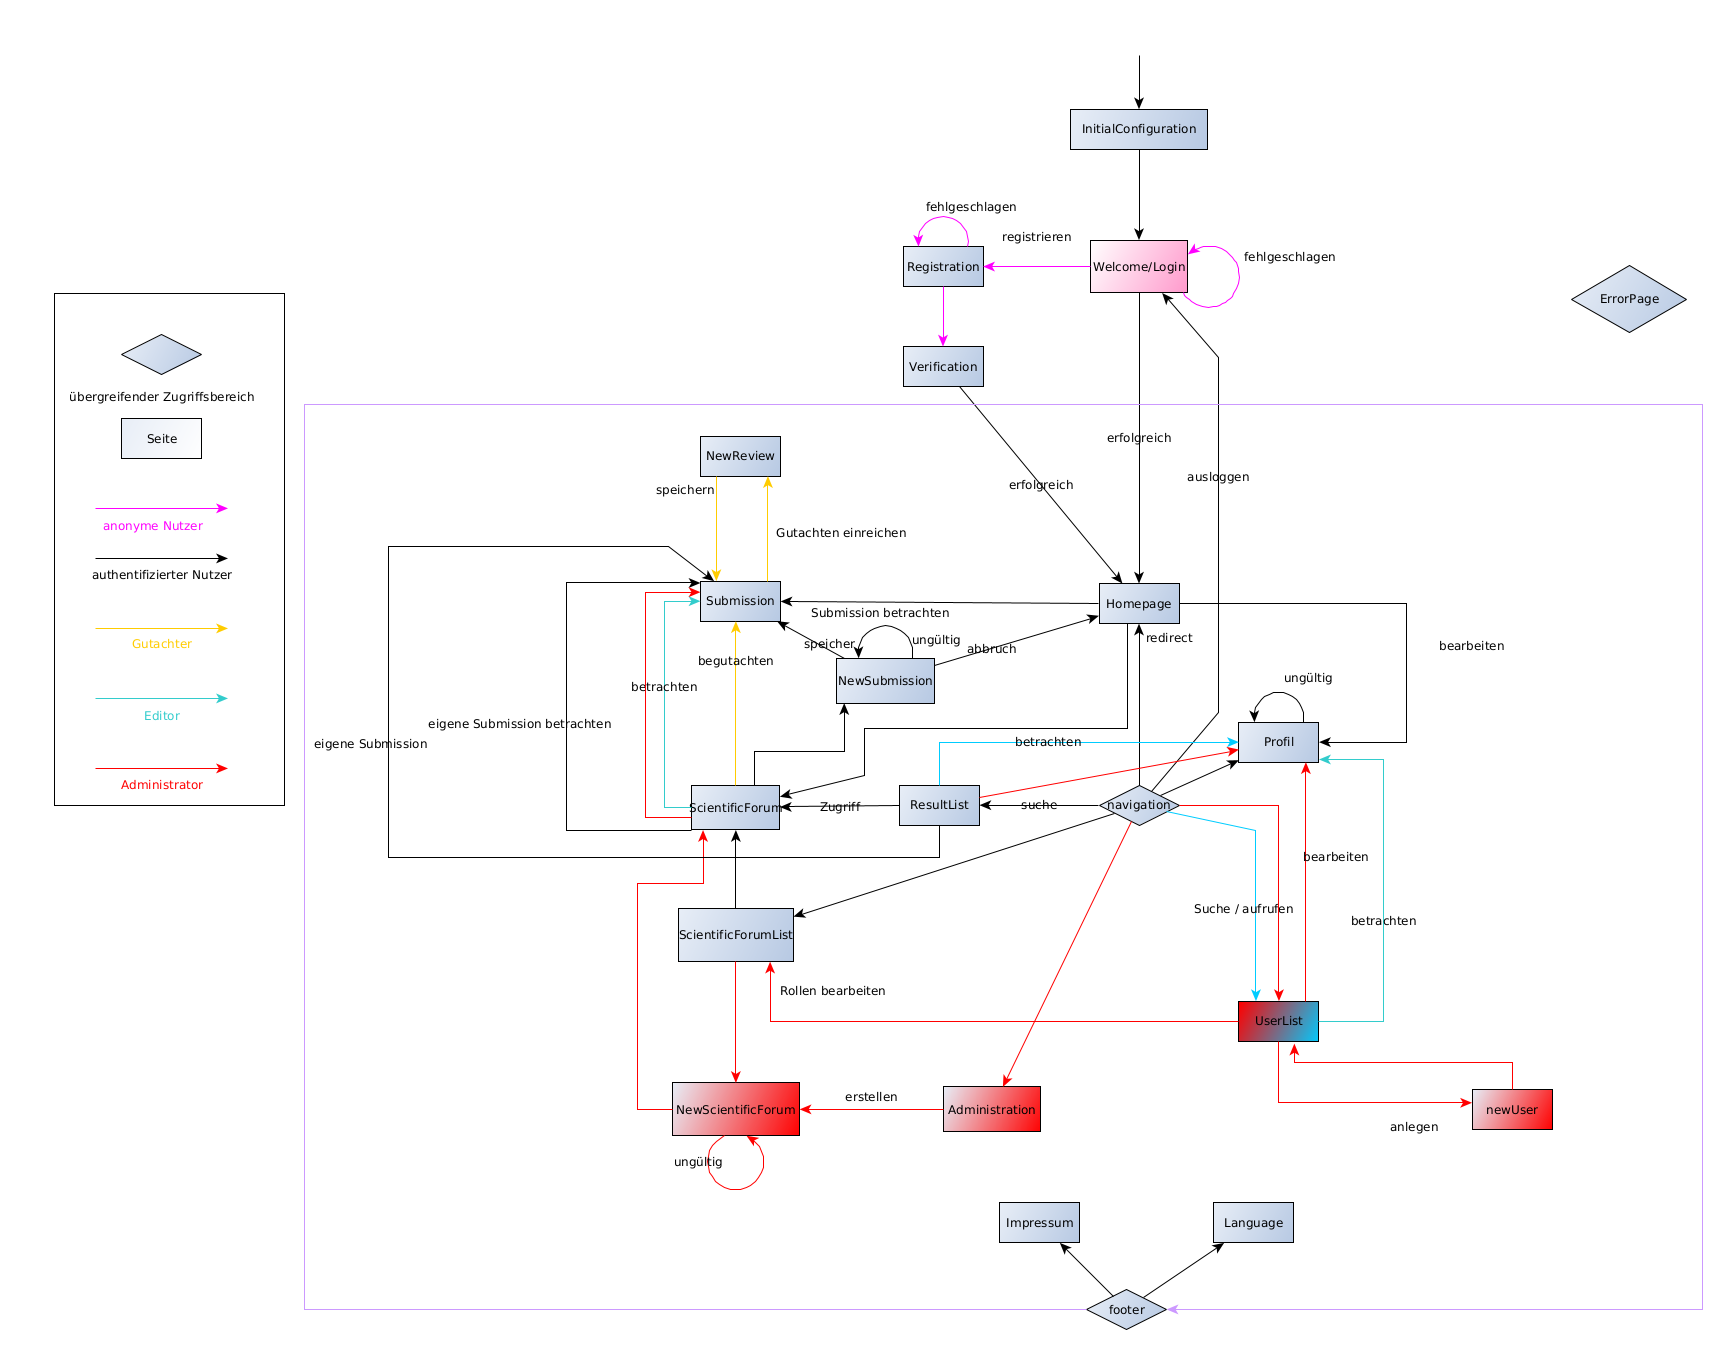
\includegraphics[width=\linewidth]{graphics/benutzerFlussyEd-png}
	\caption{Analyse der Navigationsstruktur}
	\label{fig:benutzerfluss}
\end{figure}

Die sich im Diagramm in Abbildung \ref{fig:benutzerfluss} befindlichen Rauten stellen Header (Navigationsleiste) und Footer dar.
Hierbei wird jedoch wie folgt unterschieden: Der Header ist nur für \hyperref[mkrit:angemeldet]{authentifizierte Nutzer} zugänglich,
d.h. dieser erscheint erst nach einem erfolgreichen Login und verschwindet nach dem Logout wieder.
Der Footer hingegen ist von jeder Seite der Applikation zugänglich und somit immer sichtbar.

Im Diagramm werden \hyperref[mkrit:admin]{Administratoren}, \hyperref[mkrit:editor]{Editoren}, \hyperref[mkrit:gutachter]{Gutachter} und \hyperref[mkrit:angemeldet]{normale Nutzende} unter dem allgemeinen Begriff
authentifizierte Nutzer betrachtet.
Sind die Verbindungspfeile nicht schwarz, sondern andersfarbig dargestellt, so besitzen auch nur die
dargestellten Benutzergruppen ein Zugriffsrecht oder das Recht auf eine Aktion. (Administratoren sind von dieser Regelung
ausgeschlossen.)

\subsection{Wireframe}

Die Grundstruktur der Ansichten wird in Abbildung \ref{fig:wireframe} abgebildet, welche sich auch in den folgenden Mockups in Abbildung \ref{fig:homepageMockup} und in Abbildung \ref{fig:submission} wiederspiegelt.
Inhalte mit gestrichelten Linen sind dabei nicht immer in jeder Ansicht sichtbar.

\begin{figure}[H]
	\centering
	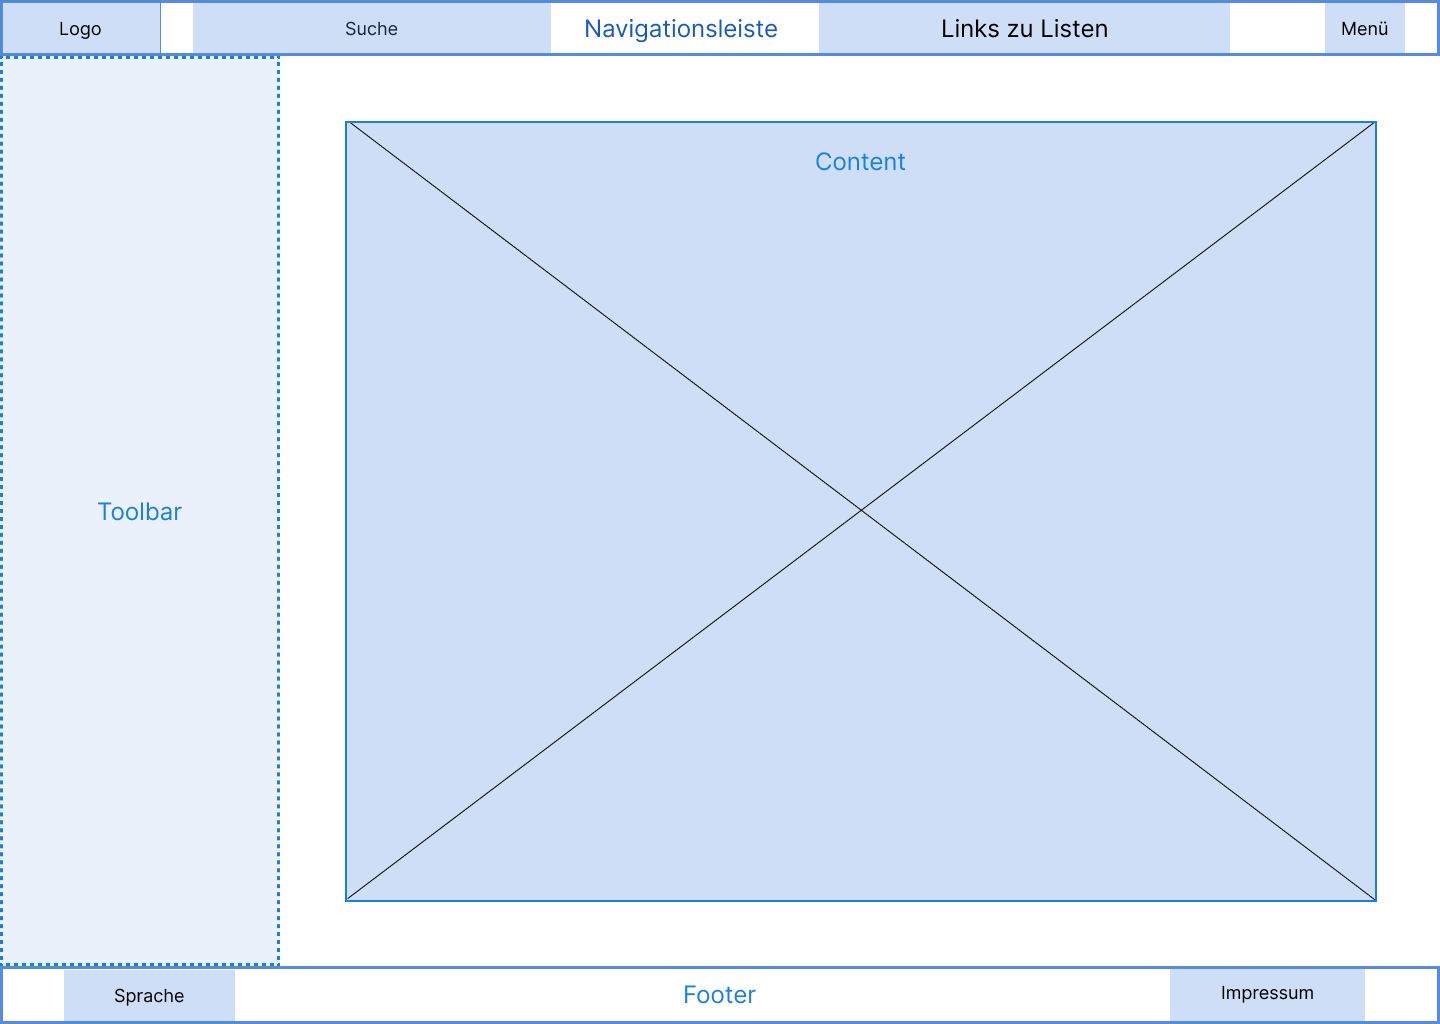
\includegraphics[width=0.85\linewidth]{graphics/Wireframe-png}
	\caption{Grundstruktur der Ansichten}
	\label{fig:wireframe}
\end{figure}

\subsection{Mockups}

Folgende Bilder zeigen einen Prototyp der Anwendung.
Dargestellt sind zwei Ausschnitte aus Schlüsselfunktionen der Webanwendung.

Die Startseite in Abbildung \ref{fig:homepageMockup} ist auf die Rolle eines \hyperref[mkrit:editor]{Editors} zugeschnitten, wobei dieser auch einige
Reviews bearbeitet und somit auch die Rolle des \hyperref[mkrit:gutachter]{Gutachters} für einige Einreichungen bekleidet.
Je nach ausgewähltem Reiter erscheinen entweder eigene, zu begutachtende Einreichungen oder Einreichungen die in eigener editorialer Verantwortung liegen.

Die Übersichtsseite der Einreichung, die Submission Seite, in Abbildung \ref{fig:submission} ist ebenfalls auf die Rolle eines \hyperref[mkrit:editor]{Editors} ausgelegt.
Ihm steht im Gegensatz zu einem \hyperref[mkrit:angemeldet]{normalen Nutzer}, welcher keine ander Rolle bekleidet, eine Toolbar zur Verfügung.
Mithilfe dieser kann er Gutachter verwalten, einen anderen \hyperref[mkrit:editor]{Editor} ernennen oder eine Revision anfordern.


\subsubsection{Startseite}

\begin{figure}[H]
	\centering
	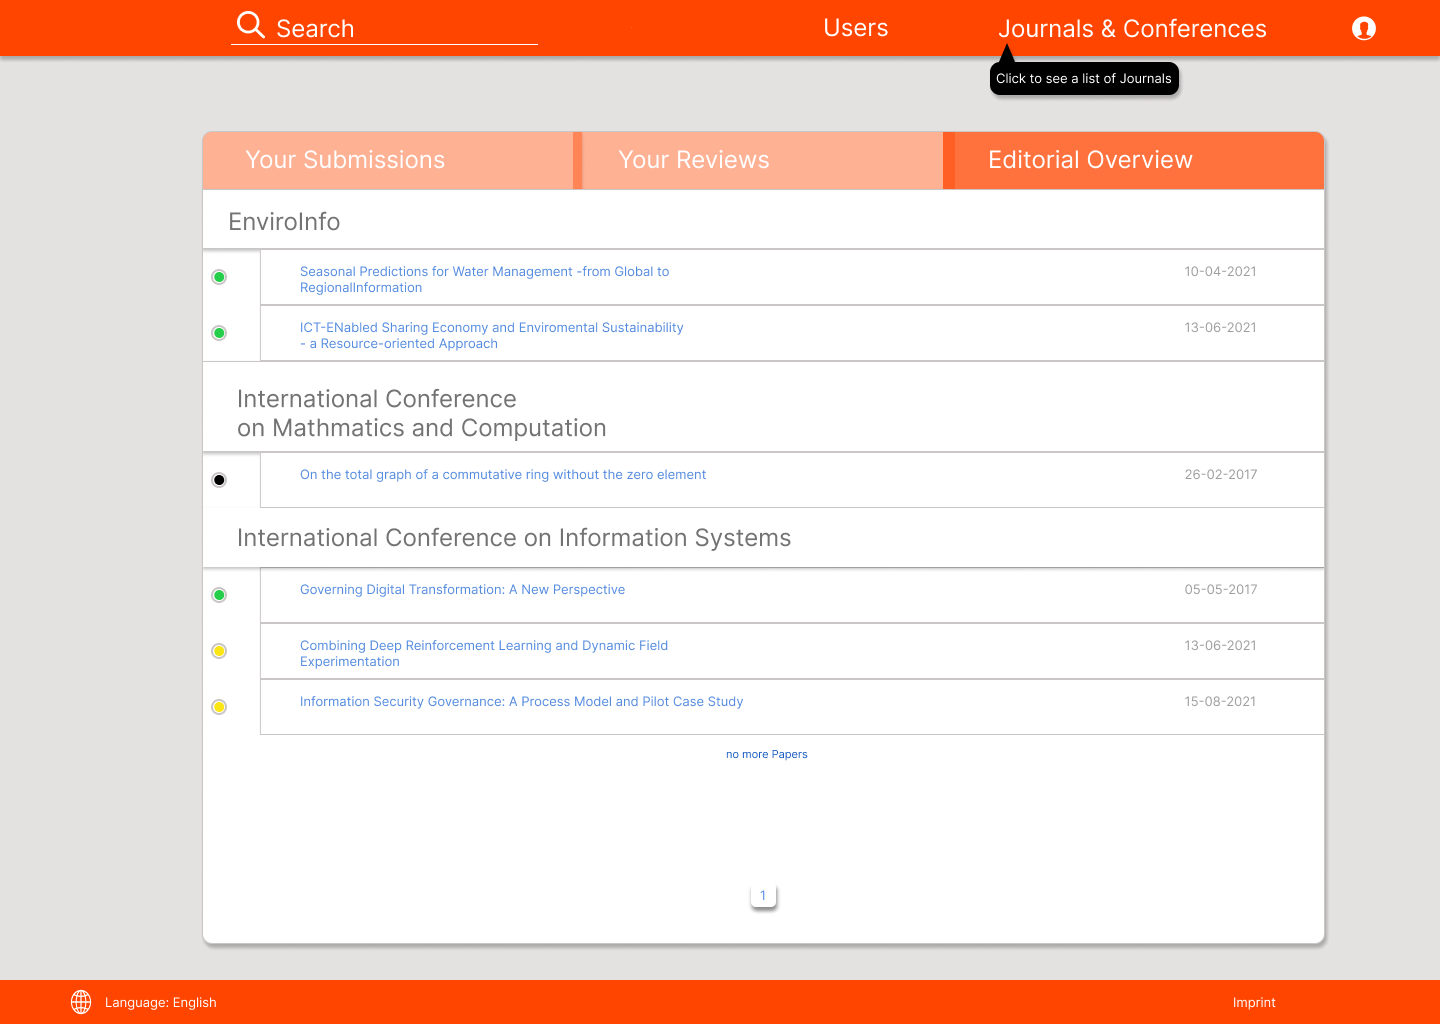
\includegraphics[width=0.85\linewidth]{graphics/Homepage-png}
	\caption{Übersicht auf einer Startseite}
	\label{fig:homepageMockup}
\end{figure}

\subsubsection{Submission}

\begin{figure}[H]
	\centering
	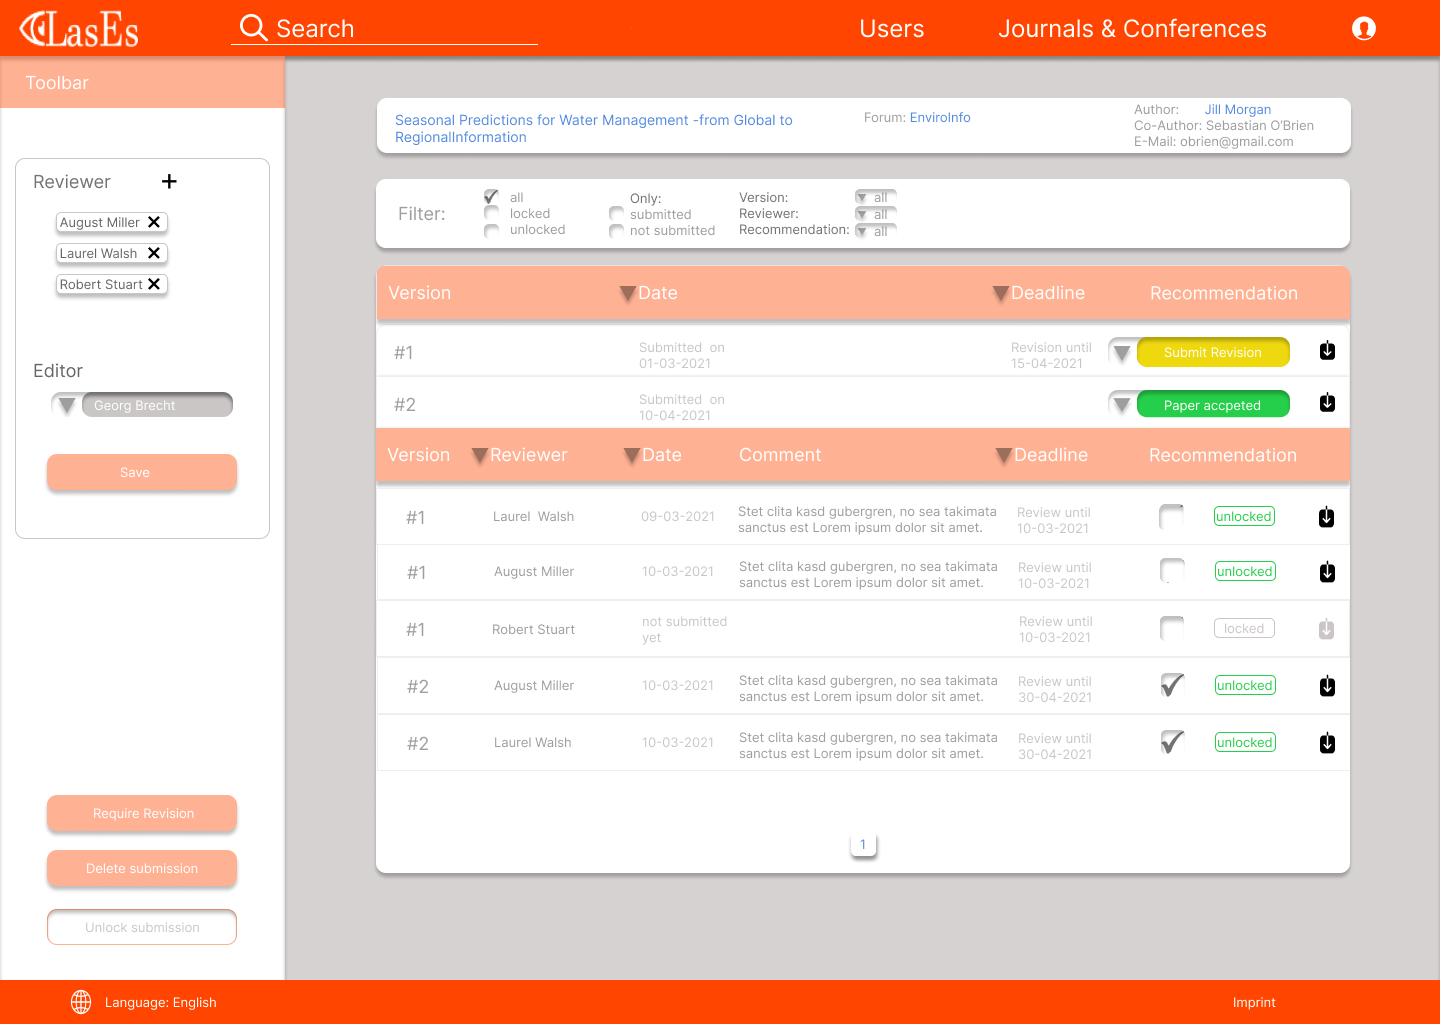
\includegraphics[width=0.85\linewidth]{graphics/Submission-png}
	\caption{Ablauf einer erfolgreichen Einreichung nach Reviews}
	\label{fig:submission}
\end{figure}

	\section{Qualitätsanforderungen}
	\localauthor{Johann Schicho}

\begin{table}[H]
	\centering
	\begin{tabular}{lccc}
		\toprule
		& zentral & wichtig & nicht im zentralen Fokus \\
		\midrule
		Mehrbenutzerbetrieb & \texttt{x} & & \\
		Robustheit & & \texttt{x} & \\
		Standardkonformität & & \texttt{x} & \\
		Benutzerfreundlichkeit & \texttt{x} & & \\
		Sicherheit & &  \texttt{x} & \\
		Erweiterbarkeit & & & \texttt{x} \\
	\end{tabular}
\end{table}

	\section{Testfälle}
	\localauthor{Sebastian Vogt}
\todo{Des nummoi erklären mit den TXXX Angelegenheiten}
\subsection{Test Setup}
Vor Ausführung jeglicher Tests sollten folgende Voraussetzungen erfüllt sein:
\begin{itemize}
	\item Das System ist vollständig eingerichtet.
	Insbesondere sind die Datenbankschemata erstellt und die globalen Einstellungen sind getroffen.
	\item Es existiert eine Administratorin mit folgenden Nutzerdaten:
	\begin{itemize}
		\item \emph{E-Mail Adresse}: kirz@fim.uni-passau.de
		\item \emph{Vorname}: Johanna
		\item \emph{Nachname}: Mayer
		\item \emph{Passwort}: UniDorfen1870!
	\end{itemize}
	\item Es existiert ein Nutzer mit folgenden Nutzerdaten:
	\begin{itemize}
		\item \emph{E-Mail Adresse}: schicho@fim.uni-passau.de
		\item \emph{Vorname}: Franz
		\item \emph{Nachname}: Huber
		\item \emph{Passwort}: TSVDorfen2001!
	\end{itemize}
	\item Es existiert eine Nutzerin mit folgenden Nutzerdaten:
	\begin{itemize}
		\item \emph{E-Mail Adresse}: vogt@fim.uni-passau.de
		\item \emph{Vorname}: Petra
		\item \emph{Nachname}: Müller
		\item \emph{Passwort}: TSVDorfen2002!
	\end{itemize}
	\item Es existiert ein Nutzer mit folgenden Nutzerdaten:
	\begin{itemize}
		\item \emph{E-Mail Adresse}: guerster@fim.uni-passau.de
		\item \emph{Vorname}: Tuti
		\item \emph{Nachname}: Aslan
		\item \emph{Passwort}: SupaDöner1970!
	\end{itemize}
\end{itemize}
Die Tests werden in der angegebenen Reihenfolge ausgeführt.
Das heißt jeder Test kann die Zustandsänderungen, die durch vorherige Tests ausgelöst worden sind, als gegeben voraussetzen.
\subsection{Administratoren}
Zuerst testen wir die Funktionen der Administratoren.
Die Einstellungen, die von der Administratorin getroffen werden, können so im Folgenden als Voraussetzungen genutzt werden.
\begin{description}

	\XXitem{/T010/}{t010} \emph{Testet \hyperref[funkt:830]{/F830/}}.
	Die Administratorin meldet sich mit ihren Anmeldedaten im System an und wird zur Startseite weitergeleitet.
	Über die Kopfzeile ruft sie nun die Liste der wissenschaftlichen Foren auf.
	Von dort aus navigiert sie zur Seite zur Erstellung eines neuen wissenschaftlichen Forums.
	Dort erstellt sie ein Forum mit folgenden Daten:
	\begin{itemize}
		\item \emph{Editor:innen}: Nutzer mit E-Mail-Adresse guerster@fim.uni-passau.de
		\item \emph{Name}: Chemie Tagung
		\item \emph{Deadline}: 30.12.2022
		\item \emph{Kurzbeschreibung}: Es geht um Chemie.
		\item \emph{URL}: ch.em.ie
		\item \emph{Anleitung zur Begutachtung}: Begutachten Sie.
	\end{itemize}
	Danach wird sie auf die Seite des wissenschaftlichen Forums weitergeleitet.

	\XXitem{/T015/}{t015} \emph{Testet \hyperref[funkt:830]{/F830/}}.
	Die Administratorin ruft über die Kopfzeile die Liste der wissenschaftlichen Foren auf.
	Von dort aus navigiert sie zur Seite zur Erstellung eines neuen wissenschaftlichen Forums.
	Dort erstellt sie ein Forum mit folgenden Daten:
	\begin{itemize}
		\item \emph{Editor:innen}: Nutzer mit E-Mail-Adresse guerster@fim.uni-passau.de
		\item \emph{Name}: Physik Tagung
		\item \emph{Deadline}: 30.12.2099
		\item \emph{Kurzbeschreibung}: Es geht um Physik.
		\item \emph{URL}: ph.ys.ik
		\item \emph{Anleitung zur Begutachtung}: Begutachten Sie.
	\end{itemize}
	Danach wird sie auf die Seite des wissenschaftlichen Forums weitergeleitet.

\end{description}

\subsection{Angemeldeter Nutzer}
\begin{description}

	\XXitem{/T020/}{t020} \emph{Testet \hyperref[funkt:160]{/F160/}}.
	Die Nutzerin mit der E-Mail-Adresse vogt@fim.uni-passau.de meldet sich im System an.
	Anschließend gibt sie im Suchfeld in der Kopfzeile ``Chemie Tagung'' ein und schickt die Suchanfrage mit Enter ab.
	Nun wird sie auf die Seite mit den Suchergebnissen weitergeleitet und das Forum namens ``Chemie Tagung'' ist der einzige Eintrag in der angezeigten Liste.
	Nach einem Klick auf diesen Eintrag wird die Nutzerin auf die Seite des wissenschaftlichen Forums weitergeleitet.

	\XXitem{/T030/}{t030} \emph{Testet \hyperref[funkt:400]{/F400/}}.
	Nun navigiert die Nutzerin per Mausklick auf die Seite für eine neue Einreichung.
	dort ist das Feld mit dem wissenschaftlichen Forum bereits richtig ausgefüllt, und zwar mit ``Chemie Tagung''

	\XXitem{/T040/}{t040} \emph{Testet \hyperref[funkt:420]{/F420/}}.
	Anschließend lädt die Nutzerin folgende PDF-Datei hoch: \href{https://dl.acm.org/doi/pdf/10.1145/3321707.3321795}{https://dl.acm.org/doi/pdf/10.1145/3321707.3321795}.

	\XXitem{/T045/}{t045} \emph{Testet \hyperref[funkt:450]{/F450/}}.
	Sie trägt in den Feldern des Formulars folgende Daten ein:
	\begin{itemize}
		\item \emph{Name der Einreichung}: Wichtiges Papier
		\item \emph{Co-Autoren}: Ein Co-Autor mit folgenden Daten:
		\begin{itemize}
			\item \emph{Vorname} Valentin
			\item \emph{Nachname} Kasper
			\item \emph{E-Mail-Adresse} garstenaue
		\end{itemize}
		\item \emph{Editor}: guerster@fim.uni-dorfen.de
	\end{itemize}
	Da die angegebene E-Mail-Adresse nicht gültig ist, ist die Registrierung nicht erfolgreich.
	Sie bleibt auf der Registrierungsseite und wird mit einer Fehlermeldung über das Problem informiert.

	\XXitem{/T050/}{t050} \emph{Testet \hyperref[funkt:410]{/F410/}}.
	Sie trägt wieder die gleichen Daten in das Formular ein wie in Test \hyperref[t050]{/T050/}, nur diesmal mit der E-Mail-Adresse \texttt{garstenaue@fim.uni-passau.de}

	\XXitem{/T060/}{t060} \emph{Testet \hyperref[funkt:460]{/F460/}}.
	Nach erfolgreicher Absendung des Formulars wird die Nutzerin auf die Übersichtsseite der Einreichung weitergeleitet.

	\XXitem{/T070/}{t070} \emph{Testet \hyperref[funkt:460]{/F460/}}.
	Frau Müller ist jetzt fertig mit ihrer Arbeit und führt mit dem zugehörigen Link in der Kopfzeile den Logout durch.
	Sie befindet sich nun wieder auf den Anmeldeseite.
\end{description}

\subsection{Editor}
\begin{description}

	\XXitem{/T080/}{t080} \emph{Testet \hyperref[funkt:680]{/F680/}}.
	Der Nutzer mit der E-Mail-Adresse guerster@fim.uni-passau.de meldet sich im System an.
	Von der Startseite aus ruft er die Einreichung ``Wichtiges Papier'' auf und landet auf der Seite dieser Einreichung.
	Er gibt in das Formular zur Zuweisung von Gutachtern ``schicho@fim.uni-passau.de'' ein und schickt das Formular ab.
	Anschließend meldet er sich ab.

	\todo{Evenutuell F690, aso die Versendung der Email noch testen...}

	\todo{F700 noch testen, aber nicht hier, sondern nach den Sachen vong Gutachter}

\end{description}

\subsection{Gutachter}
\begin{description}

	\XXitem{/T090/}{t090} \emph{Testet \hyperref[]{}}.
	Der Nutzer mit der E-Mailc-Adresse schicho@fim.uni-passau.de meldet sich im System an.
	Von der Startseite aus ruft er die Einreichung ``Wichtiges Papier'' auf und landet auf der Seite dieser Einreichung.

\end{description}

\subsection{Anonyme Nutzer}

\begin{description}
	\XXitem{/T200/}{t200} \emph{Testet \hyperref[funkt:010]{/F010/}}. Valentin Kasper aus \hyperref[t050]{/T050/} ist noch nicht im System registriert.
	Er ruft LasEs auf und wird zur Anmeldeseite weitergeleitet.
	\XXitem{/T210/}{t210} \emph{Testet \hyperref[funkt:060]{/F060/}}. Er klickt auf den Link zur Registrierung und gibt seinen Namen, seine E-Mail-Adresse und das Passwort \texttt{einsZwei3!5678} an.

	Die Registrierung wird bestätigt und er erhält eine Verifizierungs-E-Mail.
	\XXitem{/T220/}{t220} \emph{Testet \hyperref[funkt:070]{/F070/}}. Er klickt auf den Bestätigungslink in der E-Mail und wird auf die Verifizierungsseite weitergeleitet.
	Damit ist sein Profil erstellt.
	Er wird automatisch auf die Homepage weitergeleitet.
	\XXitem{/T230/}{t230} \emph{Testet \hyperref[funkt:260]{/F260/}}. Da er als Ko-Autor in Test \hyperref[t050]{/T050/} eingetragen wurde, wird ihm das Paper auf der Homepage angezeigt.
\end{description}



	\section{Entwicklungsumgebung}
	\localauthor{Sebastian Vogt}
\subsection{Programmierung}
\begin{itemize}
	\item \emph{Entwicklerrechner}: Die Entwickler verwenden folgende Systeme für die Entwicklung:
		\begin{itemize}
			\item Lenovo IdeaPad C340-14IML, Intel(R) Core(TM) i5-10210U CPU @ 1.60GHz 2.11GHz, 16GB RAM, Windows 11
			\item Lenovo IdeaPad Flex 5 14IIL05, Intel(R) Core(TM) i5-1035G1 CPU @ 1.00GHz 1.19GHz, 8GB RAM, Windows 10
			\item Acer Swift SF314-55, Intel(R) Core(TM) i5-8265U CPU @ 1.60GHz 1.80GHz, 8GB RAM, Windows 10
			\item Acer Aspire A515-54G, Intel(R) Core(TM) i5-8265U CPU @ 1.60GHz 1.80GHz, 8GB RAM, Ubuntu 20.04.3 LTS
			\item Lenovo ThinkPad E490, Intel(R) Core(TM) i5-8265U CPU @ 1.60GHz 1.80GHz, 8GB RAM, Ubuntu 20.04.3 LTS
		\end{itemize}
	\item \emph{IDE}: JetBrains IntelliJ 2021.2
	\item \emph{JDK}: Adopt-OpenJDK 16.0.2
	\item \emph{Application Server}: Tomcat 10.0.10
	\item \emph{Build Tool}: Apache Maven 3.6.3
	\item \emph{Testing Frameworks}: JUnit Jupiter 5.8.1, Selenium 3.141.59, Mockito 4.0.0
	\item \emph{In-Memory Datenbank}: H2 Database Engine 1.4.200
	\item \emph{Webbrowser}: Mozilla Firefox 93.0
	\item \emph{Mail Client}: Mozilla Thunderbird 91.2.0
\end{itemize}
Die Referenzumgebung für den Applikationsserver wird \hyperref[spezi]{hier} beschrieben.
Als Datenbankserver wird in der Entwicklung bereits der Referenzserver verwendet. Dieser wird \hyperref[dbspezi]{hier} beschrieben.
\subsection{Versionskontrolle}
\begin{itemize}
	\item \emph{Git} Version 2.25.1
	\item \emph{Zusammenarbeit} im Team wird über den \emph{GitLab} Server der Fakultät für Informatik und Mathematik der Universität Passau gehandhabt.
\end{itemize}
\subsection{Dokumente}
\begin{itemize}
	\item \emph{Textsatz}: \LaTeX
	\item \emph{\LaTeX\ Compiler}: LuaHBTeX, Version 1.13.2
	\item \emph{\LaTeX\ Distribution}: TeX Live 2021
	\item \emph{\LaTeX\ Editor}: TeXstudio 4.0.0
	\item \emph{PDF Reader}: Adobe Acrobat Reader DC 2021.007.20099, Evince 3.36.10
\end{itemize}
\subsection{Diagramme}
\begin{itemize}
	\item \emph{Klassendiagramm}: IBM Rational Software Architect 9.7 auf Debian 11
	\item \emph{Sequenzdiagramm}: PlantUML mit IntelliJ Plugin "PlantUML integration" 5.6.1
	\item \emph{Vektorgrafik Software}: Inkscape 1.1.1, Affinity 1.10.1.1142
	\item \emph{Graph Editor}: yEd 3.21.1
	\item \emph{Kollaboratives Design-Tool}: Figma Linux 0.9.2
\end{itemize}
\subsection{Orgware}
\begin{itemize}
	\item \emph{Internetanbindung} mit mindestens 1 Mbit/s Bandbreite
	\item \emph{E-Mail Dienst} der FIM mit einer ``@fim.uni-passau.de'' Adresse für jeden Entwickler und der Adresse ``sep21g02@fim.uni-passau.de'' für das gesamte Team.
\end{itemize}
\subsection{Software für Kommunikation und Organisation}
\begin{itemize}
	\item \emph{Kommunikation}: Whatsapp 2.2140.5, Discord 1.0.9003
	\item \emph{Datei Sharing}: LRZ Sync and Share
	\item \emph{Projektmanagement}: ProjectLibre 1.9.3
\end{itemize}

	\section{Glossar}
	\localauthor{Stefanie Gürster}

\begin{description}
	\XXitem{Administrator}{glo:admin} Ein Administrator ist der Betreiber und Verwalter von LasEs. Dieser kann neue \hyperref[glo:wissForum]{Wissenschaftliche Foren} erstellen und Nutzer entfernen oder hinzufügen. Ein Administrator besitzt allumfassende Rechte.

	\XXitem{Anonymer Nutzer}{glo:anon} Anonyme Nutzende sind nicht eingeloggte oder registrierte Websitenbesucher. Sie haben keinen Zugriff auf systeminterne Daten und können nur die Anmeldungs- oder Registrierungsseite sehen.

	\XXitem{Build Tool}{glo:buildtool} \href{https://maven.apache.org/what-is-maven.html}{Apache Maven} ist ein Build System für Java Anwendungen. Es erlaubt die einfache Einbindung von weiteren Softwarebibliotheken und übernimmt den Bau eines \hyperref[glo:war]{\texttt{war}} Archivs.

	\XXitem{Client}{glo:client} Rechner eines Webseitenbenutzers.

	\XXitem{CPU}{glo:cpu} \emph{Central Processing Unit} Zentrale Recheneinheit des Prozessors der Rechenbefehle ausführt.

	\XXitem{Editor}{glo:editor} Ein Editor ist einem wissenschaftlichen Forum zugewiesen und verwaltet Einreichungen.

	\XXitem{GitLab}{glo:gitlab} \href{https://fimgit.fim.uni-passau.de/users/sign_in}{GitLab} ist ein zentraler Speicherplatz für alle Entwickler. Darüber kann die Zusammenfügung einzelner Codestücke verwaltet werden.

	\XXitem{Gutachter}{glo:gutachter} Gutachter:innen können anonym die Paper anderer Wissenschaftler \emph{peer-reviewen} und Änderungen verlangen oder es als gut befinden.

	\XXitem{HTTPS}{glo:https} Protokoll zur verschlüsselten Datenübertragung über das Internet.

	\XXitem{IBM RSA}{glo:rsa} Der \emph{IBM Rational Software Architect} erlaubt \emph{Round-Trip Engineering}. Damit können gleichzeitig zur Programmierung auch die aus dem Code hervorgehenden Diagramme erstellt werden.

	\XXitem{Inkscape}{glo:inkscape} Inkscape ist ein Vektorgrafikbearbeitungsprogramm. Vektorgrafiken haben den Vorteil bei nahem \emph{heranzoomen} nicht unscharf zu werden.

	\XXitem{In-Memory Datenbank}{glo:ramdb} Zur vereinfachten Entwicklung wird während der Entwicklungsphase nicht eine echte Datenbank mit hoher Latenzzeit verwendet, sondern eine lokale Arbeitsspeicherdatenbank.

	\XXitem{IDE}{glo:ide} \emph{Integrated Development Environment} Programm, in der die Webanwendung programmiert wird und bei der Entwicklungsarbeit unterstützt.

	\XXitem{JDK}{glo:jdk} \href{https://www.oracle.com/java/technologies/downloads/}{\emph{Java Development Kit}} Komplette Softwarebibliothek der Java Programmiersprache. Enthält die Grundbausteine der Anwendung.

	\XXitem{Journal}{glo:journal} Zu einem Journal kann ein Wissenschaftler ein Manuskript in Form eines PDFs abgeben. Ein Journal hat keine Deadline zur Abgabe.

	\XXitem{JSF}{glo:jsf} \href{https://jakarta.ee/specifications/faces/}{\emph{Jakarta Server Faces}} ist das Grundgerüst von LasEs. Es erlaubt die Erstellung von Webanwendungen in der Programmiersprache Java.

	\XXitem{Konferenz}{glo:konf} Zu einer Konferenz kann ein Wissenschaftler ein Manuskript in Form eines PDFs abgeben. Eine Konferenz hat eine Deadline zur Abgabe.

	\XXitem{\LaTeX}{glo:latex} \href{https://www.latex-project.org/}{Latex} ist das Textsatzsystem zum Verfassen der Dokumente. Es ermöglicht die parallele Bearbeitung von Textdokumenten.

	\XXitem{RAM}{glo:ram} \emph{Random Access Memory} Arbeitsspeicher eines Computers. Hier sind Daten gespeichert die ein \hyperref[glo:cpu]{CPU} während der Befehlsabarbeitung benötigt.

	\XXitem{Registrierter Nutzer}{glo:regnutzer} Ein Nutzer, welcher ein Nutzerkonto erstellt hat und dieses per E-Mail verifiziert hat. Der authentifizierte Nutzer kann Papers einreichen.

	\XXitem{Pagination}{glo:pagination} Eine lange Liste mit mehr als 25 Einträgen wird auf mehrere Seiten aufgeteilt.

	\XXitem{Server}{glo:server} Rechner, auf welcher die Webanwendung ausgeführt wird und die Datenbank gespeichert ist.

	\XXitem{Submission}{glo:submission} Eine \emph{Einreichung} ist ein Manuskripts, welches auf den Datenbankserver durch den veröffentlichenden Wissenschaftler hochgeladen wird. Anschließend können Gutachter dieses Manuskript reviewen.

	\XXitem{war}{glo:war} \emph{Web Application Resource} oder \emph{Web Archive} Archivdateiformat. Bündelt die Anwendung in eine einzige Datei, die damit leicht installierbar ist.

	\XXitem{Mailto-Link}{glo:mailto} Hyperlinks über die Benutzer eine E-Mail an eine vorgegebene E-Mail-Adresse senden können, ohne diese zuvor in einem E-Mail-Programm eingeben zu müssen. Diese Mail kann eine vorgefertigte Nachricht enthalten.

	\XXitem{Wissenschaftliches Forum}{glo:wissForum} Überbegriff für \hyperref[glo:journal]{Journale} und \hyperref[glo:konf]{Konferenzen}.

	\XXitem{yEd}{glo:yed} \href{https://www.yworks.com/products/yed}{yEd} ist ein Bearbeitungsprogramm zum Erstellen von Graphen und Diagrammen.
\end{description}

\end{document}
